\chapter{Worked Example: Loop Interchange}
\label{chap:example}

\section{Original and transformed code}
Consider row-major matrices with non-overlapping storage. Both snippets compute
$C\leftarrow C+AB$. They assume that $N$ is positive, that each array has $N^2$
elements, and that index arithmetic is representable. These are original teaching
examples, not implementations reproduced from a paper.

\lstinputlisting[
  caption={Baseline matrix multiplication with an $i$--$j$--$k$ loop order.},
  label={lst:baseline}
]{code/matmul-baseline.c}

\lstinputlisting[
  caption={An $i$--$k$--$j$ loop order for the same computation.},
  label={lst:interchanged}
]{code/matmul-interchanged.c}

\Cref{lst:interchanged} advances through a row of $B$ and a row of $C$
in its innermost loop. The value $A[i,k]$ is invariant within that loop.
The diagram in \cref{fig:access-pattern} shows only the access to $B$.

\section{Explaining the access pattern}
\begin{figure}[htbp]
  \centering
  \begin{subfigure}[t]{0.48\textwidth}
    \centering
    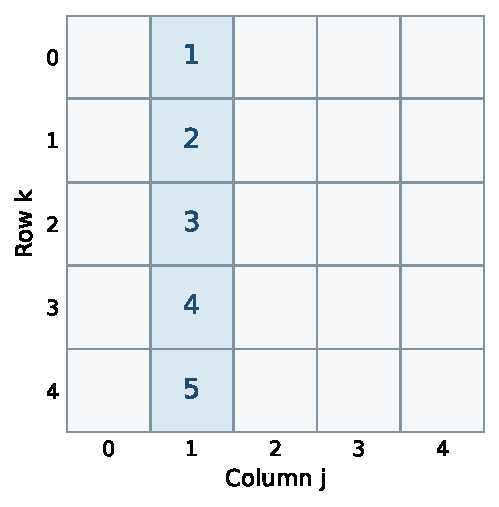
\includegraphics[width=\linewidth]{access-column.pdf}
    \caption{Fixed $j$: varying $k$ accesses a column.}
    \label{fig:column-access}
  \end{subfigure}\hfill
  \begin{subfigure}[t]{0.48\textwidth}
    \centering
    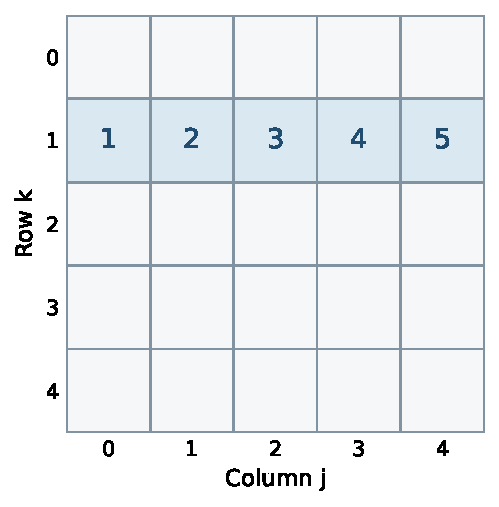
\includegraphics[width=\linewidth]{access-row.pdf}
    \caption{Fixed $k$: varying $j$ accesses a row.}
    \label{fig:row-access}
  \end{subfigure}
  \caption{Illustrative accesses to a row-major matrix $B$. Numbers indicate
  access order. The grid represents array elements, not cache lines.}
  \label{fig:access-pattern}
\end{figure}

For row-major storage, the byte offset of $B[k,j]$ is
\begin{equation}
  \operatorname{offset}(B[k,j]) = e(kN+j).
  \label{eq:row-major}
\end{equation}
Increasing $k$ by one changes the offset by $eN$, whereas increasing $j$ by one
changes it by $e$. This stride comparison explains a locality opportunity;
it is not a measured performance result.

\section{Legality and profitability}
For this example, distinct $(i,j)$ pairs update distinct elements of $C$ and
$A$ and $B$ are read-only. Each output element retains the ascending order of
$k$ contributions. Non-aliasing is therefore an essential assumption in this
explanation. Actual compiler transformations must also respect the applicable
floating-point rules. Compare results using a stated tolerance if arithmetic
contraction or other floating-point optimisations differ between builds.

A transformed loop can also change register use, vectorisation opportunities,
and instruction counts. Assess its profitability through a stated model or
measurements rather than assuming that smaller strides guarantee a speedup.
\todo{Extend this example with tiling, fusion, or skewing from your own analysis.}
